\documentclass[border=10pt]{standalone}
\usepackage{circuitikz}
\usepackage{tikz}
\usetikzlibrary{calc, positioning, arrows.meta, shapes.geometric}

\begin{document}
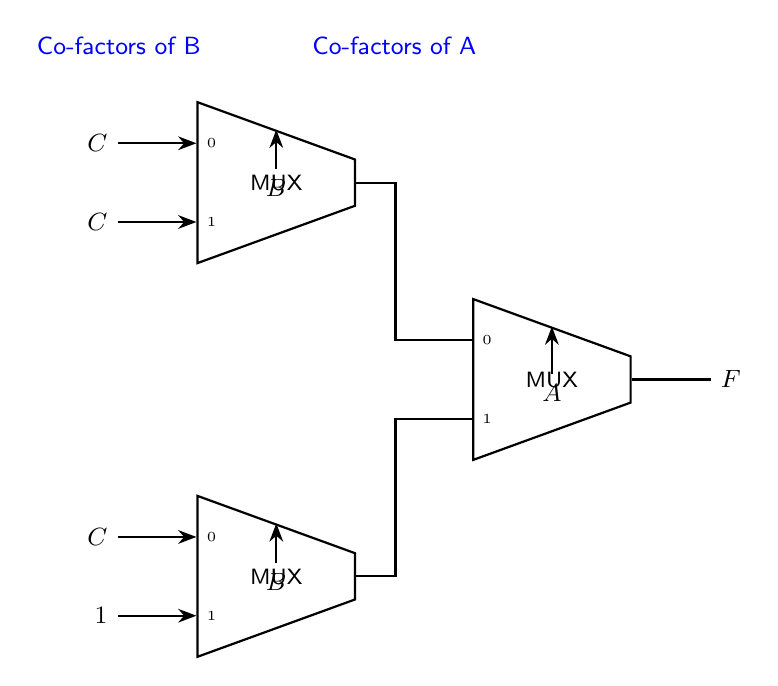
\begin{tikzpicture}[
    >=Stealth, 
    thick, 
    font=\sffamily\small
]

    % Define Trapezoidal MUX style
    % Use 'rotate=-90' to orient the trapezium with narrow side (output) to the Right.
    % 0 deg: Top (short) is Up. Bottom (long) is Down.
    % -90 deg: Top is Right. Bottom is Left.
    \tikzset{mux2to1/.style={
        draw, 
        trapezium, 
        trapezium angle=70, 
        rotate=-90,
        minimum width=1.0cm, 
        minimum height=2.0cm, 
        inner sep=0pt
    }}

    % Level 1 MUX (A)
    \node[mux2to1] (M1) at (0, 0) {\rotatebox{90}{\footnotesize MUX}};
    
    % Select Input (A)
    % Node is rotated -90.
    % .south was Bottom. Now it is Left?
    % Let's use geographic anchors of the unrotated shape, which rotate with the node.
    % .south anchor of the shape (which is the bottom side) is now at the Left?
    % Wait. 
    % 0 deg: South is Bottom.
    % -90 deg: South is Left.
    % But we want Select at Bottom of the diagram.
    % In the rotated frame:
    % -90 deg rotation means local x points down, local y points right?
    % Let's verify anchors.
    % If I use 'rotate=-90', the anchor .south (relative to page) might correspond to .west (relative to shape)?
    % No, TikZ anchors rotate with the node shape.
    % Original .south (bottom side) -> rotates to Left (West).
    % Original .west (left side) -> rotates to Bottom (South).
    % Original .east (right side) -> rotates to Top (North).
    % Original .north (top side/short side) -> rotates to Right (East).
    
    % So:
    % Output (Narrow side) is original Top (.north) -> Now at Right (East). Correct.
    % Inputs (Wide side) is original Bottom (.south) -> Now at Left (West). Correct.
    % Select should be on one of the slanted sides.
    % Side 1 (West originally) -> Bottom.
    % Side 2 (East originally) -> Top.
    % We want select at Bottom. So we use the original West anchor?
    
    % Let's use specific calculated points relative to .center to be safe if anchors are confusing.
    
    % M1 Output
    \draw (M1.north) -- ++(1, 0) node[right] {$F$}; % .north (shape) is at Right (Page East).

    % M1 Select (A)
    % Located at original West (now Bottom).
    \draw[<-] (M1.west) -- ++(0, -0.6) node[below] {$A$}; 

    % M1 Inputs (Wide Side = original South = now Left)
    \coordinate (M1_In0) at ($(M1.south) + (0, 0.5)$); % Top of diagram (y+)
    \coordinate (M1_In1) at ($(M1.south) + (0, -0.5)$); % Bottom of diagram (y-)
    
    \node[right, font=\tiny] at (M1_In0) {0};
    \node[right, font=\tiny] at (M1_In1) {1};


    % Level 2 MUXs (B)
    \node[mux2to1] (M2_0) at (-3.5, 2.5) {\rotatebox{90}{\footnotesize MUX}}; 
    \draw[<-] (M2_0.west) -- ++(0, -0.5) node[below] {$B$}; % Select B
    
    \node[mux2to1] (M2_1) at (-3.5, -2.5) {\rotatebox{90}{\footnotesize MUX}}; 
    \draw[<-] (M2_1.west) -- ++(0, -0.5) node[below] {$B$}; % Select B

    % Wiring M2 -> M1
    % M2_0 Output (north -> Right) -> M1 Input 0
    \draw (M2_0.north) -- ++(0.5, 0) |- (M1_In0);
    
    % M2_1 Output (north -> Right) -> M1 Input 1
    \draw (M2_1.north) -- ++(0.5, 0) |- (M1_In1);
    
    % M2 Inputs (south -> Left)
    \coordinate (M2_0_In0) at ($(M2_0.south) + (0, 0.5)$);
    \coordinate (M2_0_In1) at ($(M2_0.south) + (0, -0.5)$);
    \node[right, font=\tiny] at (M2_0_In0) {0};
    \node[right, font=\tiny] at (M2_0_In1) {1};

    \coordinate (M2_1_In0) at ($(M2_1.south) + (0, 0.5)$);
    \coordinate (M2_1_In1) at ($(M2_1.south) + (0, -0.5)$);
    \node[right, font=\tiny] at (M2_1_In0) {0};
    \node[right, font=\tiny] at (M2_1_In1) {1};

    % Wiring Inputs
    \draw[<-] (M2_0_In0) -- ++(-1, 0) node[left] {$C$};
    \draw[<-] (M2_0_In1) -- ++(-1, 0) node[left] {$C$};
    
    \draw[<-] (M2_1_In0) -- ++(-1, 0) node[left] {$C$};
    \draw[<-] (M2_1_In1) -- ++(-1, 0) node[left] {$1$};

    % Labels
    \node[above, blue] at (-2, 4) {Co-factors of A};
    \node[above, blue] at (-5.5, 4) {Co-factors of B};

\end{tikzpicture}
\end{document}
